% !TEX root = chapter-standalone.tex
\section{The category~\Pos of posets and monotone maps}
In this section, we want to abstract the concept of poset and describe a category in which the objects are posets themselves, and the morphisms are monotone functions between them. This category is called~\Pos.

\begin{ctdefinition}[Category \Pos]
  \label{def:Pos}
  The category~\iindex{\Pos} is defined by:
  \begin{compactenum}
    \item \emph{Objects}: The objects of this category are all posets.
    \item \emph{Morphisms}: The morphisms from a poset~$\Obja$ to a poset~$\Objb$ are the monotone maps from~$\Obja$ to~$\Objb$.
    \item \emph{Identity morphism}: The identity morphism for the poset~$\Obja$
    is the identity map~$\catid_\Obja$.
    \item \emph{Composition operation}: The composition operation is composition of maps.
  \end{compactenum}
\end{ctdefinition}

Occasionally we will write~$f \colon \Obja \toinPos \Objb$ to emphasize that a monotone map between posets is a morphism in \Pos.

\subsection{Why~\Pos is not sufficient for design theory}

\todo{Rewrite this without assuming we know what is a design problem.}
The category \Pos of posets and monotone maps that we have described can model many facts that are useful for design theory. However, there are also limitations which motivate us to describe a more general category. This section describes the usefulness and the limitations of~\Pos.

\begin{example}[Battery]
  Consider a model of a battery where the capacity is the functionality and the mass of the battery is the resource.
%(\cref{fig:battery-example}).
  There is certainly a monotone map from capacity to mass. This map answers the question: ``Given a value of the capacity, what is the minimum mass needed?''. Conversely, in the other direction, the map that answers the question: ``Given a certain mass, what is the maximum capacity that can be provided?'' is also a monotone map.
\end{example}

\begin{comment}
  \begin{figure}[h!]
    \centering
    \begin{tikzcd}
      \bullet &\arrow[l] \bullet\\[-15pt]
      \text{mass} & \text{capacity}
    \end{tikzcd}
    \caption{Example of the design of a battery. }
    \label{fig:battery-example}
  \end{figure}
\end{comment}

Therefore, at first sight it might seem that posets and monotone maps would be sufficient to describe a quantitative theory of design. However, there are more general relations to be modeled. It is easy enough to describe examples in which having a simple monotone map from functionality to resources is not sufficient.

\begin{example}[Delivery drone]
  Consider the design of a delivery drone, in which the functional requirement is that the drone should be able to make a delivery at a distance~$d$ and we need to reason about how powerful to make the drone. In particular, we need to choose at what (average) \emph{velocity}~$v$ the drone should travel and what is the optimal \emph{mission duration}. The relation between distance~$d$, velocity~$v$, and mission duration~$T$ is given by~$d=v\cdot T$. We can choose to have either a fast drone and short missions, or a slow drone and long missions. This is an interesting trade-off. Flying fast takes more energy, both for propulsion as well as for computation (more objects to be observed and processed). Flying too slow will also be excessively energy-consuming because of the long mission duration.

  If we consider~$v$ and~$T$ as given, then the map~$\tup{v,T} \mapsto v\cdot T$ is clearly a monotone function that gives the distance which the drone can cover. However, in the other direction, we do not have a simple map, but rather a 1-to-many relation $\mathrm{distance}\to \mathrm{velocity}\times \mathrm{time}$. For each fixed value of the distance, there is an entire continuum of values of~$v$ and~$T$ which we can choose, as it can be seen in~\cref{fig:drone-example-antichain}.

  \begin{figure}[h!]
    \centering
    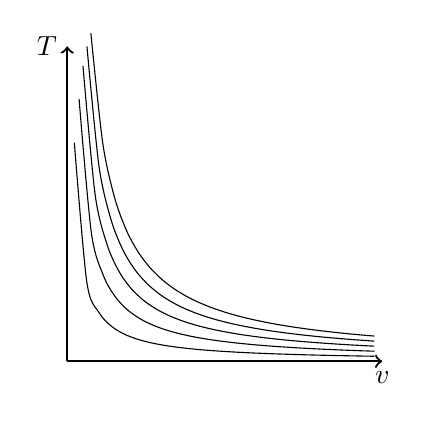
\begin{tikzpicture}
      \draw[->, thick] (0,0)--(4,0) node[below]{$v$};
      \draw[->, thick] (0,0)--(0,4) node[left]{$T$};
      \draw[domain=0.3:3.9,smooth,variable=\t]plot (\t,1.25/\t);
      \draw[domain=0.25:3.9,smooth,variable=\t]plot (\t,1/\t);
      \draw[domain=0.2:3.9,smooth,variable=\t]plot (\t,0.75/\t);
      \draw[domain=0.15:3.9,smooth,variable=\t]plot (\t,0.5/\t);
      \draw[domain=0.09:3.9,smooth,variable=\t]plot (\t,0.25/\t);
    \end{tikzpicture}
    \caption{Antichains in~$\tup{v,T}$ for different values of~$d$.}
    \label{fig:drone-example-antichain}
  \end{figure}

\end{example}

In other words, using~\Pos it is not possible to make a theory of \emph{trade-offs}. We will introduce a more general category, called the category~\DP of \emph{design problems} (\cref{sec:dpdefinition}), which will allow to describe such a theory.

\devel{\GZ{Check with JL what he means.}}


